\ifdefined\withimages
	\newpage
	\tikz[remember picture,overlay] \node[opacity=1,inner sep=0pt] at (current page.center){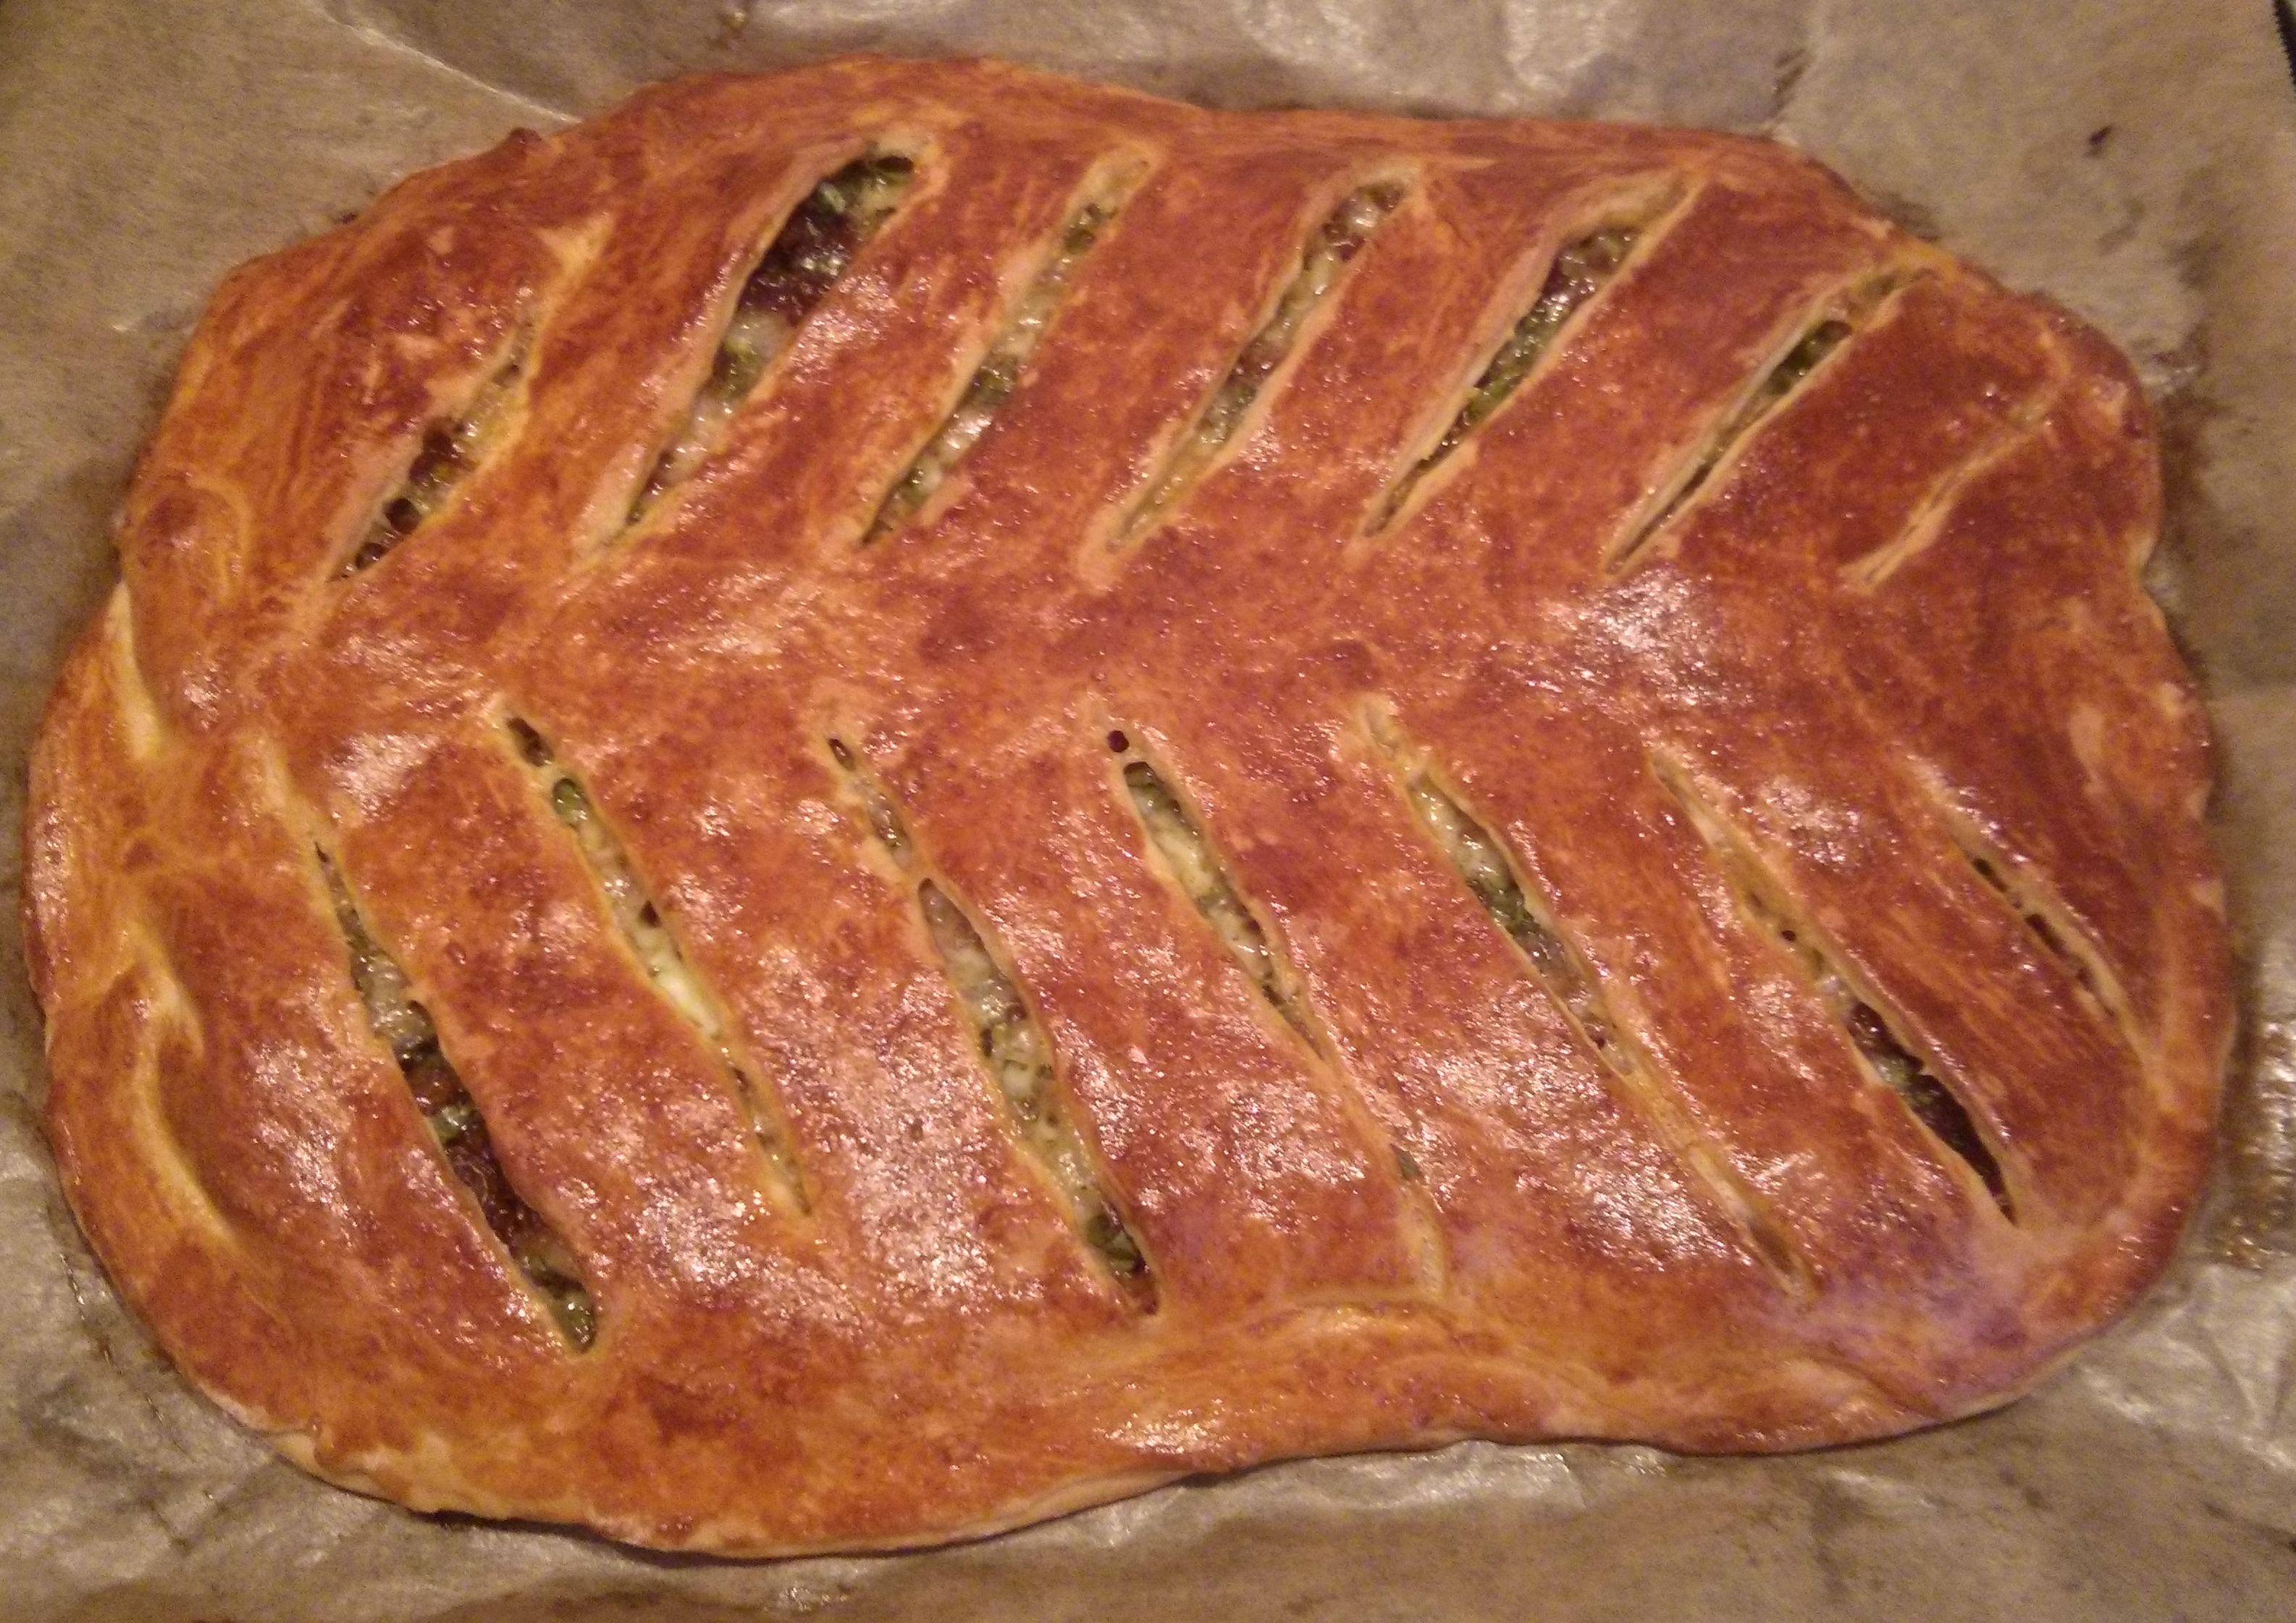
\includegraphics[width=\paperwidth,height=\paperheight]{./bilder/gefueltes_brot_ratio.jpg}};
\fi

\begin{recipe}[]{Gefülltes Brot} %Josi
	\timerecipe[Minuten]{ca. 15 + 60 + 15 + 30} %mit [EINHEIT]
	\personcount{2-3} % mit[ART]
	\ingredient{300g Mehl} % ggf. \nicefrac{1}{2}
	\ingredient{15g frische Hefe}
	\ingredient{150g gekocheter Schinken}
	\ingredient{1 Bund Petersilie}
	\ingredient{2 Knoblauchzehen}
	\ingredient{1 Kugel Mozzarella}
	\ingredient{50g getrocknete Tomaten}
	\ingredient{1 Eigelb}

\step \textbf{15g Hefe} und \textbf{eine Prise Zucker} in 160ml lauwarmen Wasser lösen und mit \textbf{1\nicefrac{1}{2} EL Olivenöl}, \textbf{1 TL Salz} und \textbf{300g Mehl} zu einen glatten Teig kneten. 

\step Den Teig ca. eine Stunden an einem warmen Ort gehen lasse.

\step Den Backofen auf 200 Grad Ober-/Unterhitze vorheizen.

\step \textbf{150g gekochten Schinken} in Streifen schneiden, \textbf{1 Bund Petersilie} und \textbf{2 Knoblauchzehen} fein hacken und  \textbf{50g getrockneten Tomaten} und \textbf{eine Kugel Mozzarella} würfeln. Mischen und mit \textbf{Salz} und \textbf{Pfeffer} würzen.

\step Den Teig in zwei Fladen ausrollen und auf dem einen die Masse bis an den Rand verteilen. Nun den zweiten Fladen kreuzweise einschneiden und auf dem ersten an drücken und mit \textbf{einem Eigelb} bepinseln.

\step 20-25 Minuten auf mittlerer Schiene backen und noch lauwarm essen.

%\tippbox{{Tipp:} ...} % Tipp in extra Rahmen
\end{recipe}